%% V1.0
%% by Gabriel Garcia, gabrcg@gmail.com
%% This is a template for Udacity projects using IEEEtran.cls

%% Be Udacious!

\documentclass[10pt,journal,compsoc]{IEEEtran}

\usepackage[pdftex]{graphicx}    
\usepackage{cite}
\usepackage{hyperref}
\hyphenation{op-tical net-works semi-conduc-tor}


\begin{document}

\title{Where Am I}

\author{Ghee Chong Foo}

\markboth{Localization project, Robotics Nanodegree Program, Udacity}%
{}
\IEEEtitleabstractindextext{%

\begin{abstract}

This write up is about creating ROS (Robot Operating System) package such as to develop mobile robot model and simulate under Gazebo environment.  The robot models were then integrated with AMCL (Adaptive Monte Carlo Localization) and Navigation stack, in particular move\_base ROS package to localize and direct the robot to a goal position in provided map.  Parameters corresponding to each package are then added or tuned in order to achieve desired result.  A benchmark robot model was first used for base line performance evaluation, and student robot model was then developed for comparison.  Both benchmark robot and student robot model were able to reach the goal, with some performance lag for student robot model.

\end{abstract}

% Note that keywords are not normally used for peerreview papers.
\begin{IEEEkeywords}
Robotics, Udacity, \LaTeX, Localization.
\end{IEEEkeywords}}


\maketitle
\IEEEdisplaynontitleabstractindextext
\IEEEpeerreviewmaketitle
\section{Introduction}
\label{sec:introduction}

\IEEEPARstart
{L}ocalization is an important topic for mobile robots to determine its position based on sensor observations such as camera and range sensor.  However noisy sensor input and uncertainty in the environment poses tremendous challenges for the mobile robots.  Multiple algorithm has been developed to filter measurement and process noise, including Kalman Filters and Particle Filters.  For this project, particle filter was chosen for its ease of implementation and robustness, but with the cost of being more resource intensive.  

%{T}{he} introduction should provide some material regarding the history of the problem, why it is important and what is intended to be achieved. If there exists any previous attempts to solve this problem, this is a great place to note these while conveying the differences in your approach (if any). The intent is to provide enough information for the reader to understand why this problem is interesting and setting up the conversation for the solution you have provided
%Use this space to introduce your localization task and how you wish to accomplish it; save the details about the robot construction for later (simulation is a good point for this information). 
%If you have any papers / sites / repositories you have referenced for your robot, please make sure to cite them.

%example for inserting image
\begin{figure}[thpb]
      \centering
      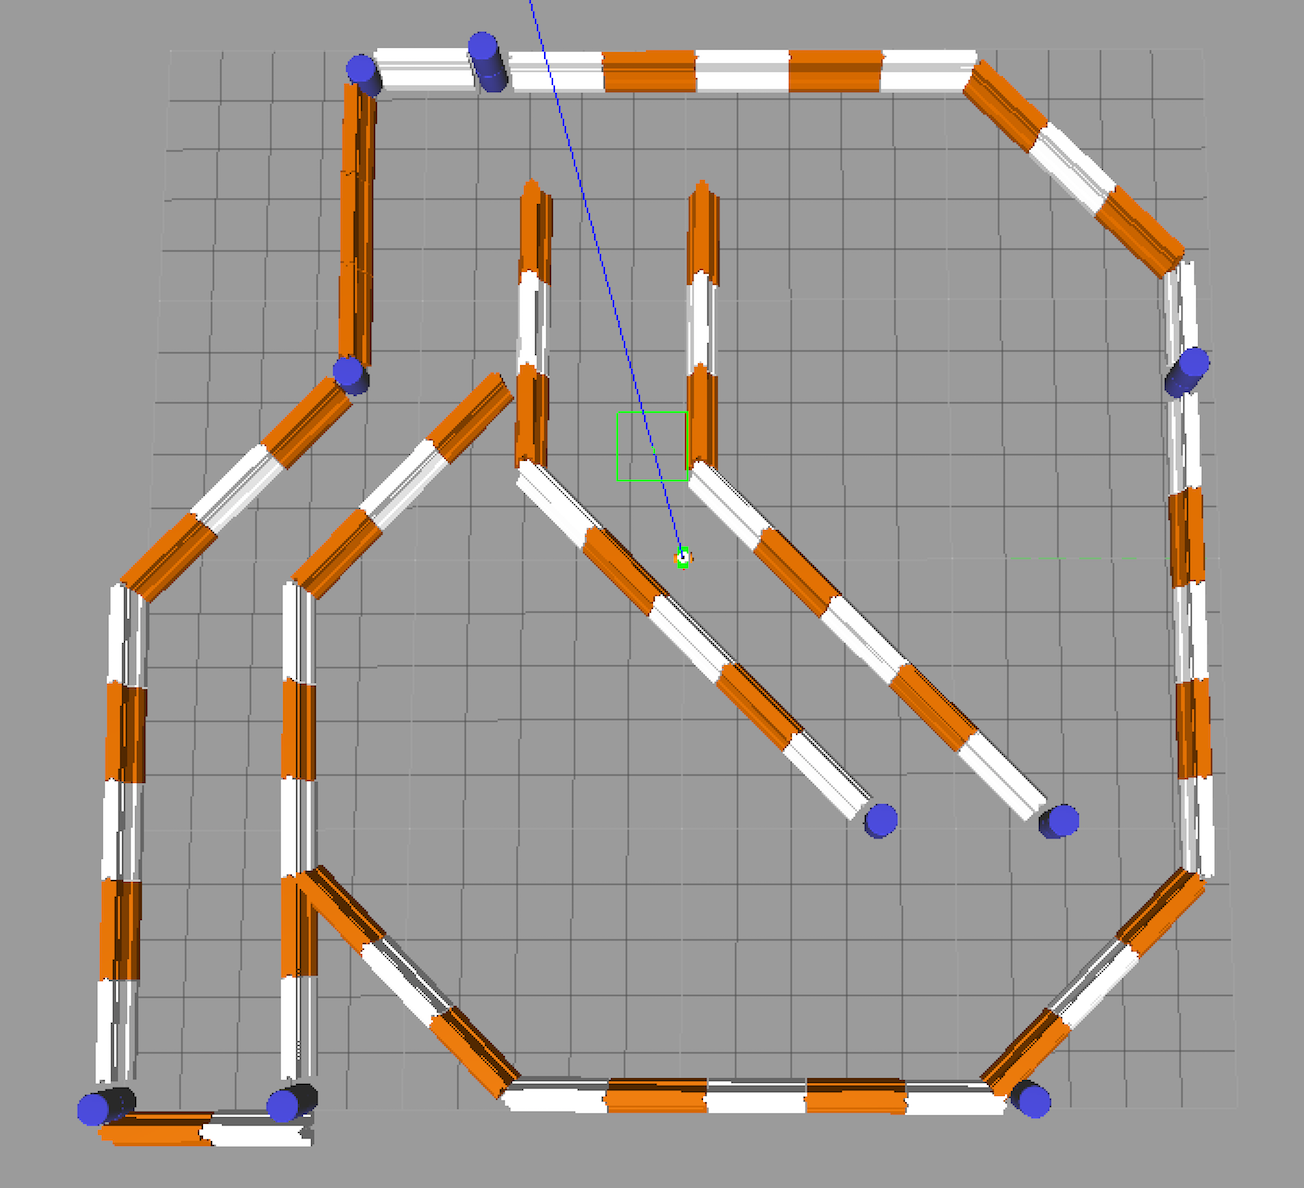
\includegraphics[width=\linewidth]{where_am_i}
      \caption{Jackal Race Map}
      \label{fig:Map}
\end{figure}

%\subsection{Subsection Heading Here}
%Subsection text here.

%\subsubsection{Subsubsection Heading Here}
%Subsubsection text here.

%example for building table
%\begin{table}[h]
%\caption{Table}
%\label{table_example}
%\begin{center}
%\begin{tabular}{|c||c|}
%\hline
%One & Two\\
%\hline
%Three & Four\\
%\hline
%\end{tabular}
%\end{center}
%\end{table}



%\section{Background}
%At this stage, you should begin diving into the technical details of your approach by explaining to the reader what are the characteristics of the filters, what localization method was chosen, and the reason that it was selected (i.e. particle filters). 
%This should be factual and authoritative, meaning you should not use language such as "I think this will work" or "Maybe Monte Carlo Localization with these parameters is better...". Instead, focus on items similar to, "Adaptive Monte Carlo Localization was chosen because..."

%Provide a sufficient background into the scope of the problem technologically while also identifying some of the current challenges in robot localization and why the problem domain is an important piece of robotics.\cite{lamport1994latex}

%\subsection{Kalman Filters}
%Briefly describe Kalman filters. Explain how they work and why they are used for localization. Additionally, discuss the drawbacks of linear Kalman filters and how Extended Kalman Filters (EKFs) help resolve some of these issues.

%\subsection{Particle Filters}
%Briefly explain what a particle filter is, how it is used, and why it is useful.

%\subsection{Comparison / Contrast}
%Explain the benefits and disadvantages of using a Kalman Filter / Particle Filter. Why would you use one over the other? Also inform the reader that the work presented here will be using only particle filters. 

%example for Bullet point list
%\begin{itemize}
%\item example 1
%\item example 2
%\end {itemize}

%example for numbered list
%\begin{enumerate}
%\item example 1
%\item example 2
%\end{enumerate}

\section{Simulations}
%This section should discuss the performance of robots in simulation. Items to include are the robot model design, packages used, and the parameters chosen for the robot to properly localize itself. The information provided here is critical if anyone would like to replicate your results. After all, the intent of reports such as these are to convey information and build upon ideas so you want to ensure others can validate your process.
%You should have at least two images here: one that shows your standard robot used in the first part of the project, and a second robot that you modified / built that is different from the first robot. Remember to watermark all of your images as well. \cite{lamport1994latex}

Two robots models was developed under ROS environment.  Both robots are able to navigate and reach the goal position through the maze within 5 minutes.  Result varies depending on running on own machine (MacBook Pro) or Udacity provided workspace, the later has GPU enabled and had much stable performance, and hence all simulation results were based on Udacity workspace.

%\subsection{Achievements}
%You should describe what you achieved for localization in the project with the benchmark model and your own model. Includes charts and graphs show how parameters affect your performance. 

% Robot Models
\subsection{Benchmark Model}

\begin{figure}[thpb]
      \centering
      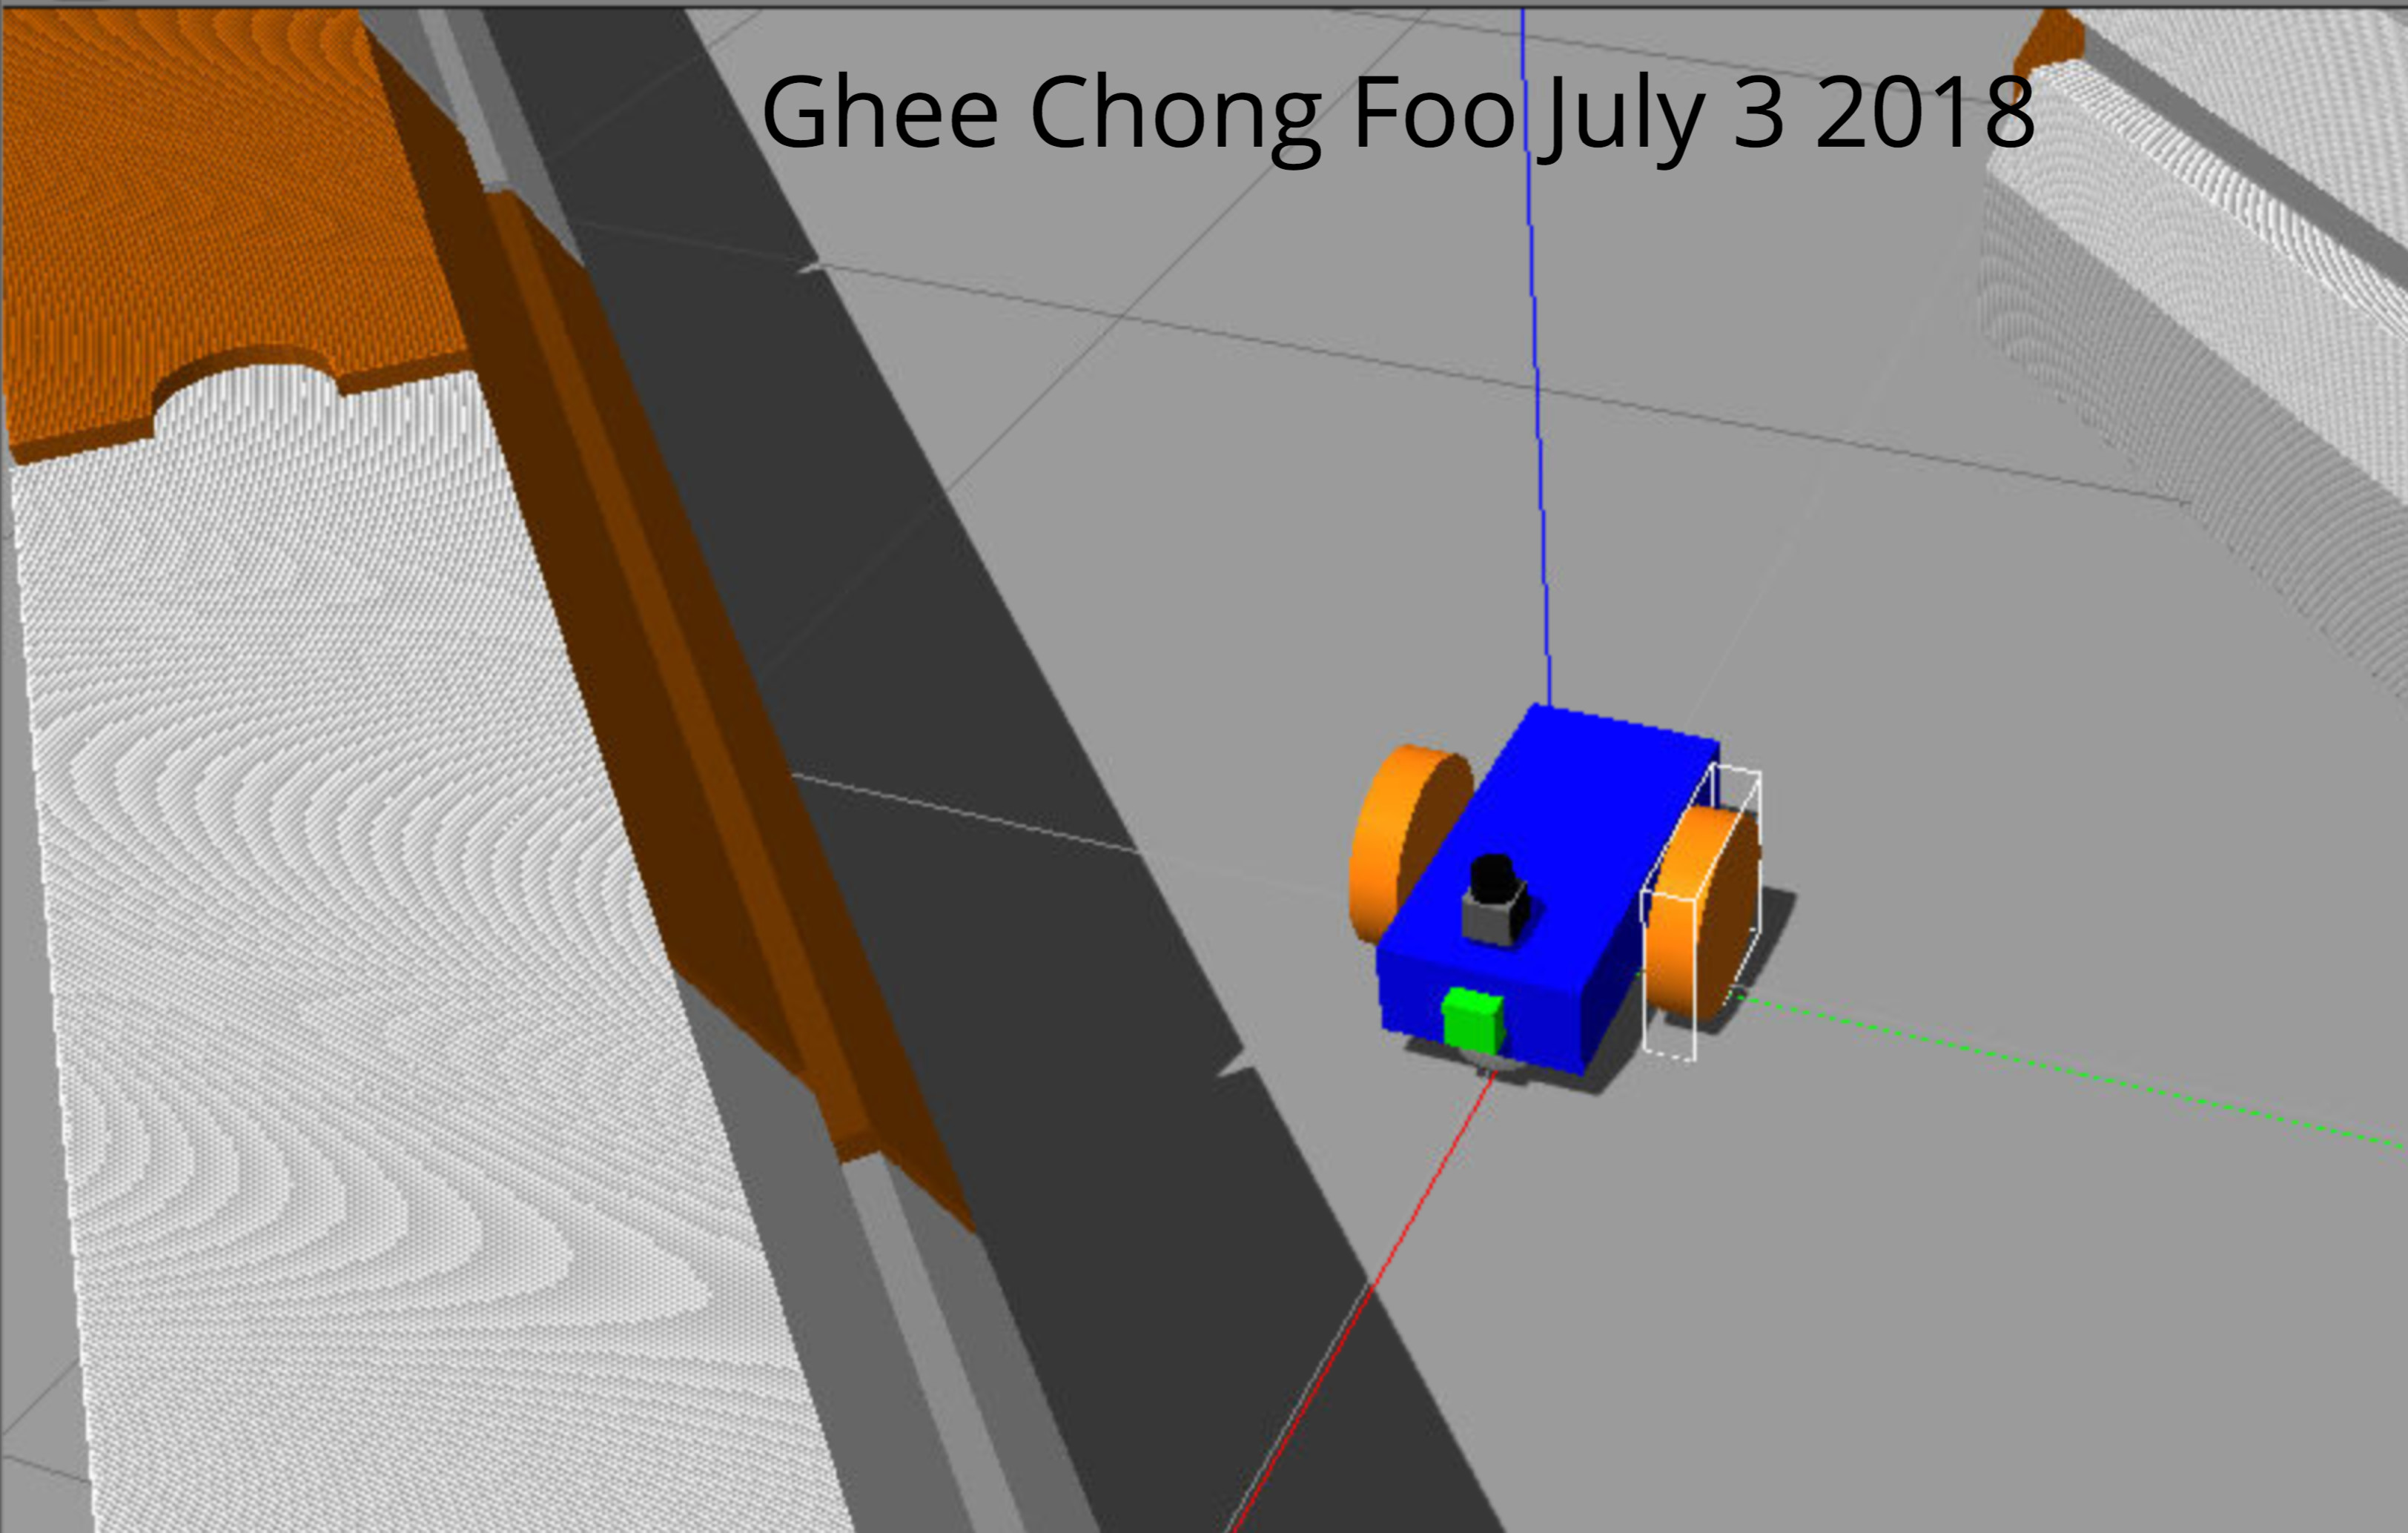
\includegraphics[width=\linewidth]{udacity_bot}
      \caption{udacity\_bot}
      \label{fig:udacity_bot}
\end{figure}

\subsubsection{Model design}
%The Robot's design considerations should include: the size of the robot, the layout of sensors. This information can be shown in the form of a chart / table.
A benchmark model was provided by Udacity, which was a 2-wheel robot on a rectangular chassis with an RGB sensor at the front, and Hokuyo laser range finder mount at the front top of the chassis, as depicted in Fig. ~\ref{fig:udacity_bot}

\subsubsection{Packages Used}
%The packages used in the project should be specified as well as the topics received and published; the services it used and provided should also be addressed. 
The following ROS package were utilized:
\begin{enumerate}
\item AMCL
\item move\_base

\end {enumerate}

\subsubsection{Topics received and published}
Below is the list of non-default topics that is received and published based on "rostopic list" output:
\begin{itemize}
\item /amcl
\item /initialpose
\item /joint\_states
\item /map
\item /odom
\item /particlecloud
\item /tf
\item /udacity\_bot/camera1
\item /udacity\_bot/laser/scan

\end {itemize}

\subsubsection{Parameters}
%Localization parameters in the AMCL node should be described, as well as move\_base parameters in the configuration file. You should be able to clearly demonstrate your understanding of the impact of these parameters.
Critical parameters that had significant influence on robot model's performance are listed and discussed as below.  Parameters definition was refer from \cite{costmap_2d}.

Table ~\ref{Costmap Common Parameters}:
\begin{table}[h]
\setlength{\tabcolsep}{1pt}  %GC this makes the table fit the page
\caption{Costmap Common Parameters}
\label{Costmap Common Parameters}
\begin{center}
\begin{tabular}{|c||c|}
\hline
Parameter & Value\\
\hline
obstacle\_range & 2.0\\
\hline
raytrace\_range & 3.0\\
\hline
transform\_tolerance & 0.2\\
\hline
footprint & [[-0.22, -0.20], [-0.22, 0.20], [0.22, 0.20], [0.22, -0.20]] \\
\hline
inflation\_radius & 0.4\\
\hline
\end{tabular}
\end{center}
\end{table}

Referring to Table \ref{Costmap Common Parameters}, the parameters were tuned to match the size of the robots, also for proper visualization of world map, global costmap and local costmap.

Table ~\ref{Base Local Planner Parameters}:
\begin{table}[h]
\setlength{\tabcolsep}{1pt}  %GC this makes the table fit the page
\caption{Base Local Planner Parameters}
\label{Base Local Planner Parameters}
\begin{center}
\begin{tabular}{|c||c|}
\hline
Parameter & Value\\
\hline
controller\_frequency & 10.0\\
\hline
\end{tabular}
\end{center}
\end{table}

Referring to Table \ref{Base Local Planner Parameters}, controller\_frequency was reduced to prevent "Control Loop Missed" error message.

Table ~\ref{Global Costmap Parameters}:
\begin{table}[h]
\setlength{\tabcolsep}{1pt}  %GC this makes the table fit the page
\caption{Global Costmap Parameters}
\label{Global Costmap Parameters}
\begin{center}
\begin{tabular}{|c||c|}
\hline
Parameter & Value\\
\hline
update\_frequency & 1.0\\
\hline
publish\_frequency & 1.0\\
\hline
\end{tabular}
\end{center}
\end{table}

Referring to Table \ref{Global Costmap Parameters}, update\_frequency and publish\_frequency were lowered to 1.0 so as not to over-stress the system and churning out "Map update loop" missed error message.

Table ~\ref{Local Costmap Parameters}:
\begin{table}[h]
\setlength{\tabcolsep}{1pt}  %GC this makes the table fit the page
\caption{Local Costmap Parameters}
\label{Local Costmap Parameters}
\begin{center}
\begin{tabular}{|c||c|}
\hline
Parameter & Value\\
\hline
update\_frequency & 1.0\\
\hline
publish\_frequency & 1.0\\
\hline
width & 5.0\\
\hline
height & 5.0\\
\hline
\end{tabular}
\end{center}
\end{table}

Referring to Table \ref{Local Costmap Parameters}, as in Global Costmap, a lower update\_frequency and publish\_frequency of 1.0 was set so only lower processing power was required.  Also width and height were reduced to 5.0 so that robot can be more certain of its local costmap and thus its whereabout.

Table ~\ref{AMCL Parameters}:
\begin{table}[h]
\setlength{\tabcolsep}{1pt}  %GC this makes the table fit the page
\caption{AMCL Parameters}
\label{AMCL Parameters}
\begin{center}
\begin{tabular}{|c||c|}
\hline
Parameter & Value\\
\hline
min\_particles & 50\\
\hline
max\_particles & 2000\\
\hline
odom\_alpha1-4 & 0.002\\
\hline
initial\_pose\_x & 0.0\\
\hline
initial\_pose\_y & 0.0\\
\hline
initial\_pose\_a & 0.0\\
\hline
\end{tabular}
\end{center}
\end{table}

Referring to Table \ref{AMCL Parameters}, min and max particles was reduced to meet hardware constraint of the system.  odom\_alpha value 1 through 4 which define noise level expected from the robot's movements/motions during navigation inside the map, is reduced to 0.002.  Initial pose of the robot is at the center of the map, and was setup accordingly.


\subsection{Personal Model}

\begin{figure}[thpb]
      \centering
      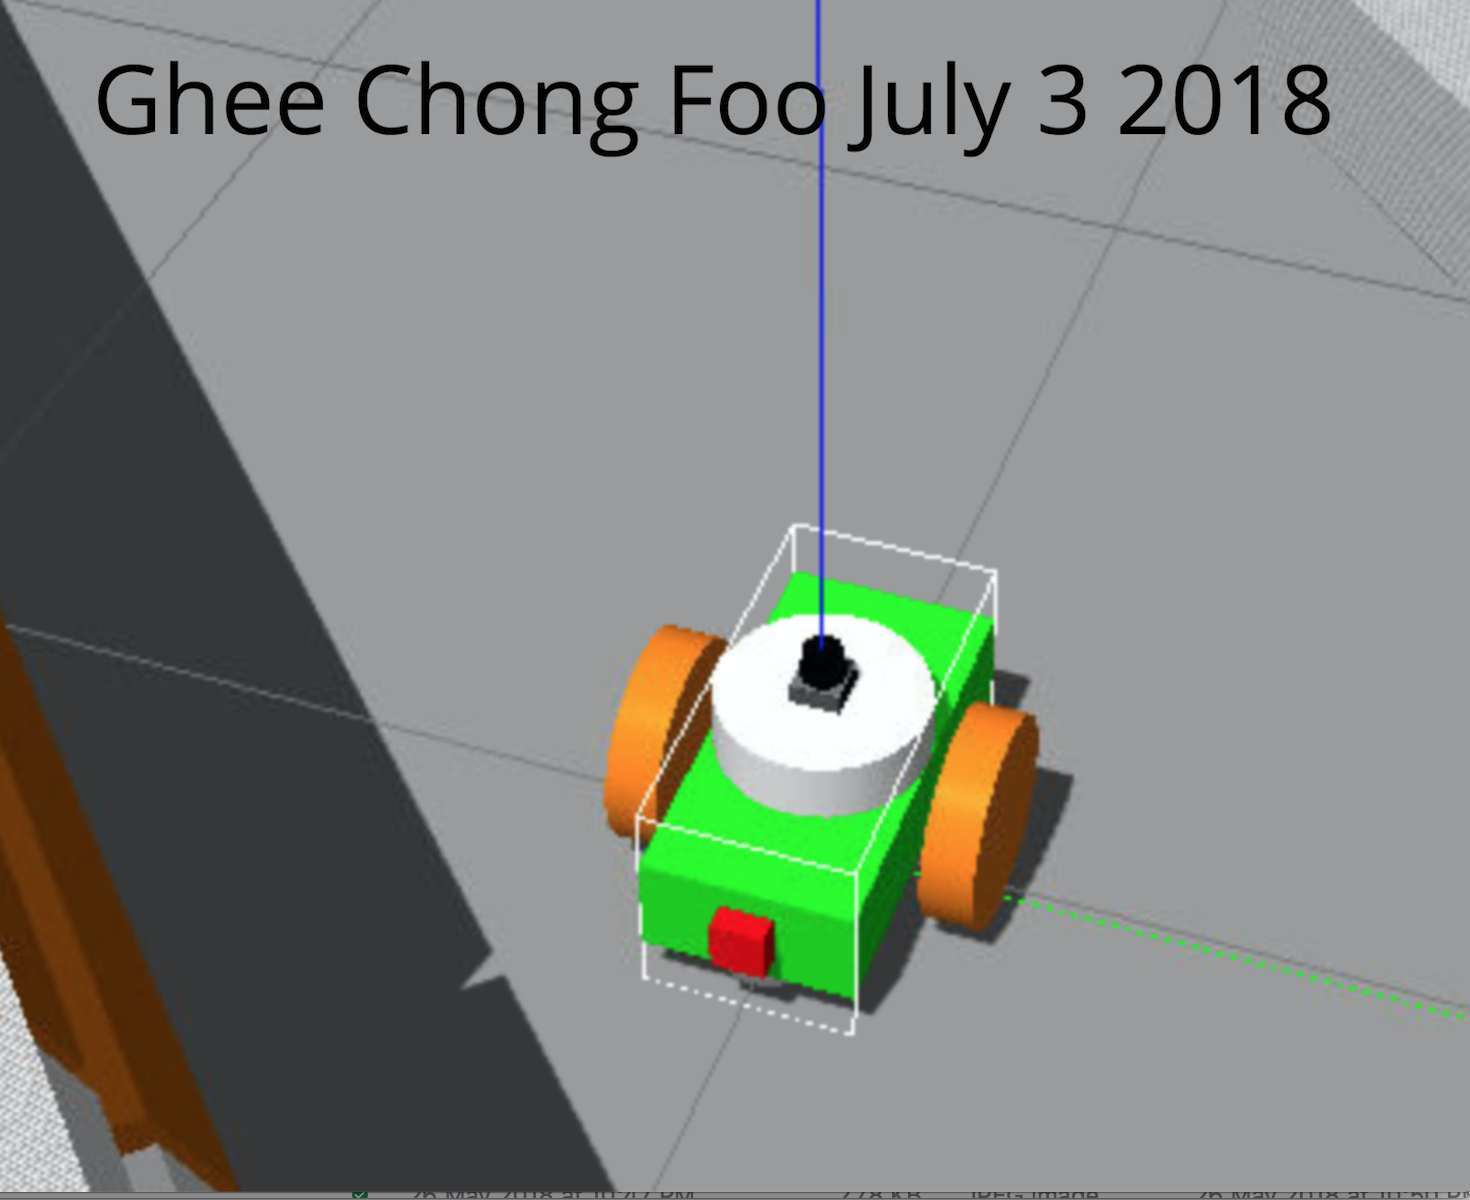
\includegraphics[width=\linewidth]{GC_bot}
      \caption{GC\_bot}
      \label{fig:GC_bot}
\end{figure}

The personal model is named GC\_bot, after the author, as depicted in Figure ~\ref{fig:GC_bot}

\subsubsection{Model design}
GC\_bot is based on the benchmark model, with additional cylinder placed on top of the chassis, and moved the Hokuyo sensor on top of the cylinder so that the sensor has a better view of the environment, this is depicted in \ref{fig:GC_bot}.

\subsubsection{Packages Used}
Same package was used as in benchmark model.
\subsubsection{Parameters}
Since similar form factor between benchmark and student model, same parameters was used.

\section{Results}
%Present an unbiased view of your robot's performance and justify your stance with facts. Do the localization results look reasonable? What is the duration for the particle filters to converge? How long does it take for the robot to reach the goal? Does it follow a smooth path to the goal? Does it have unexpected behavior in the process? \\
%For demonstrating your results, it is incredibly useful to have some watermarked charts, tables, and/or graphs for the reader to review. This makes ingesting the information quicker and easier.

\subsection{Localization Results}
\subsubsection{Benchmark}

\begin{figure}[thpb]
      \centering
      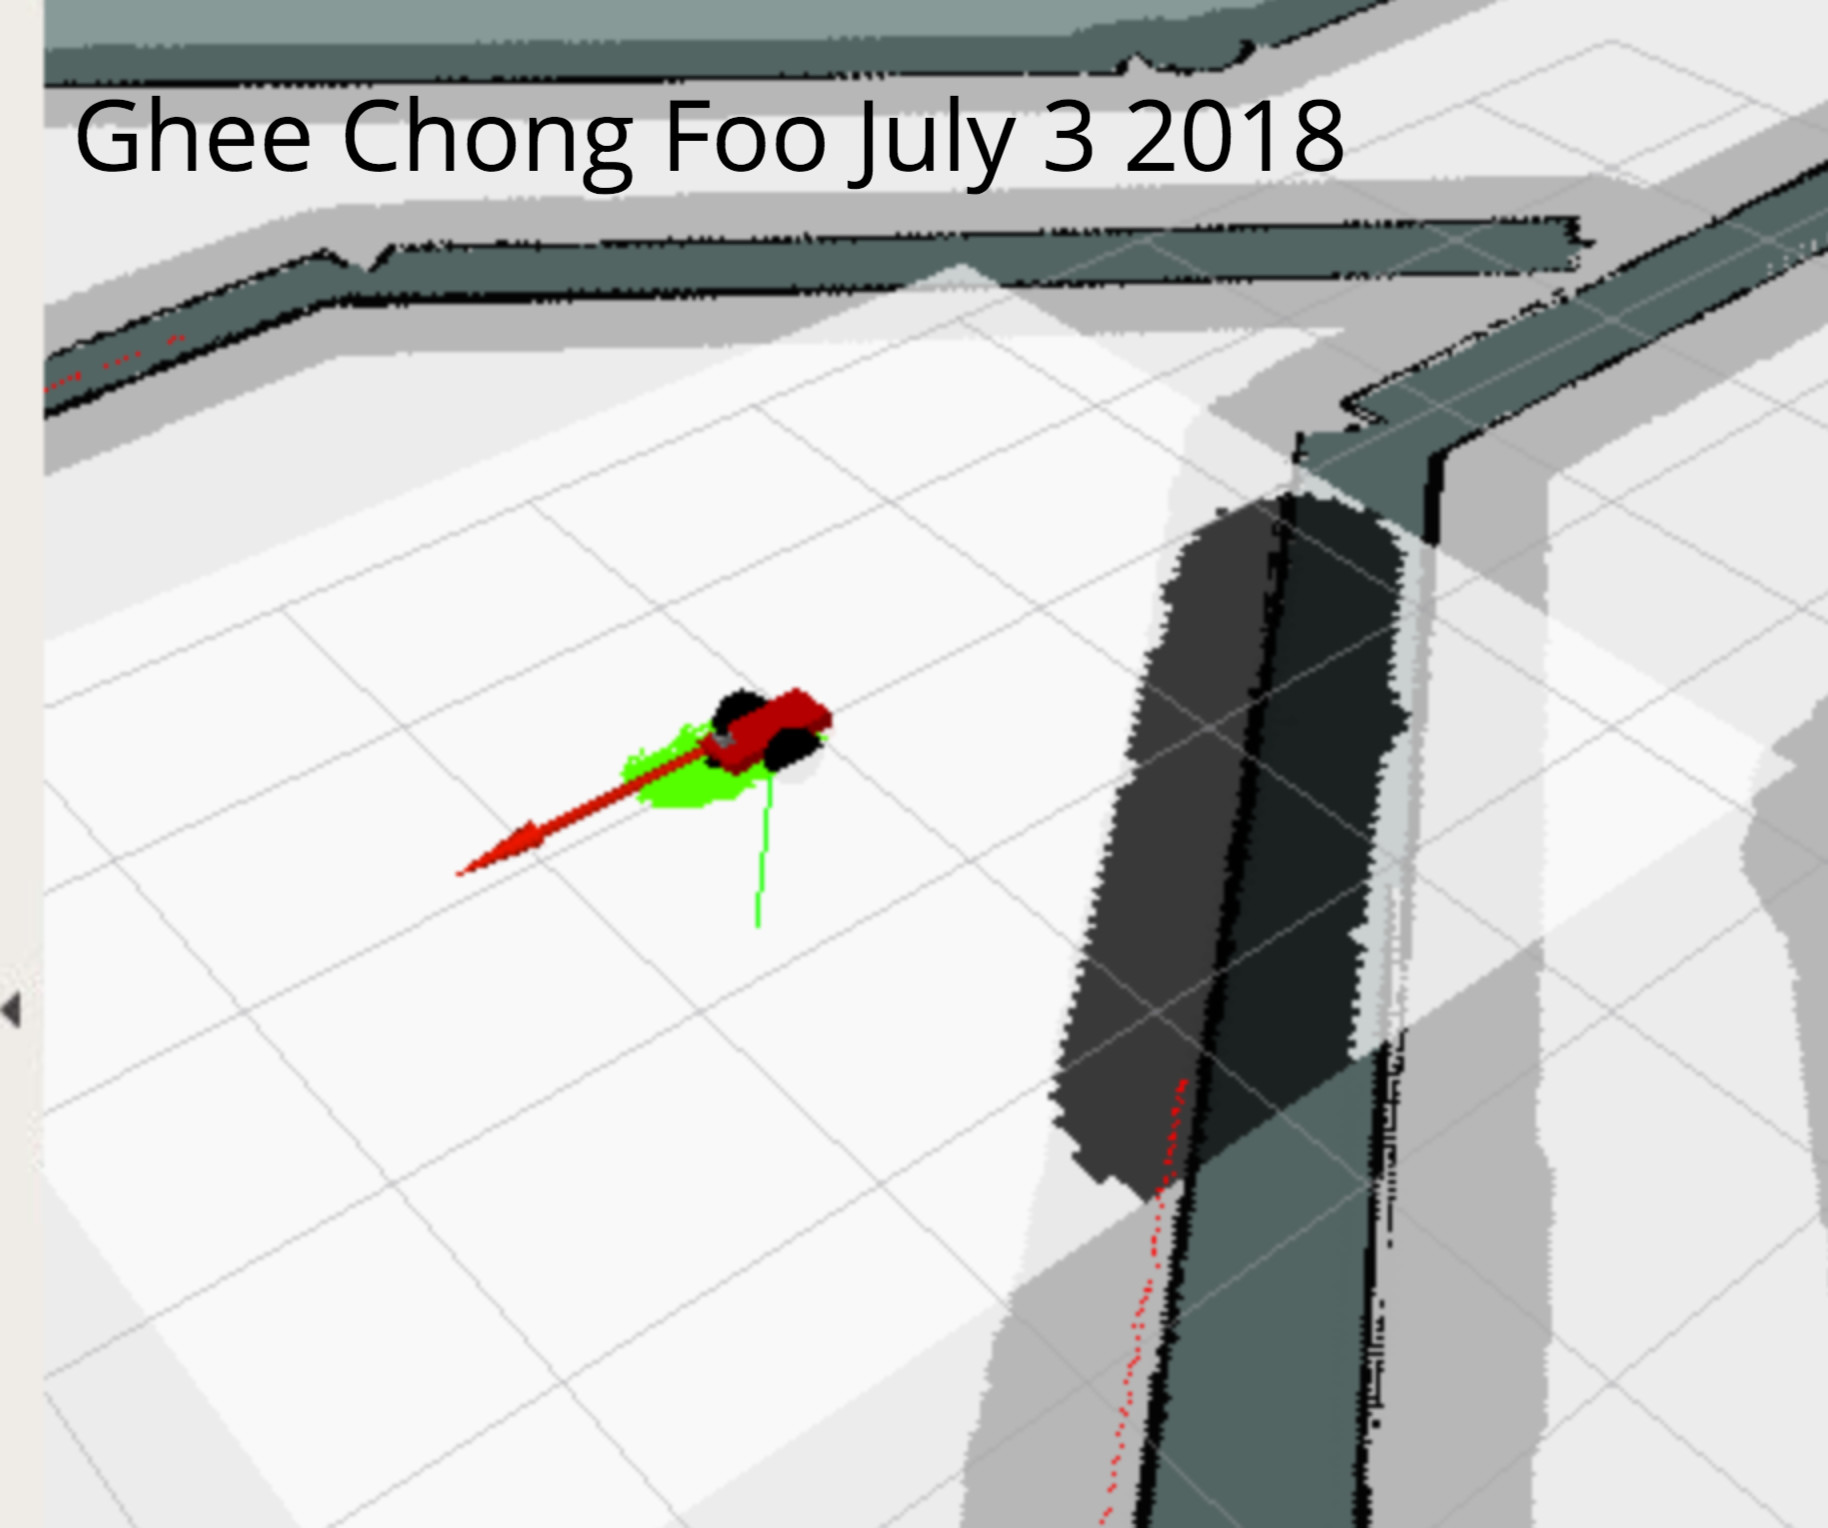
\includegraphics[width=\linewidth]{udacity_bot_reach_goal_rviz}
      \caption{udacity\_bot reached goal Rviz view}
      \label{fig:udacity_bot_reach_goal_rviz}
\end{figure}

\begin{figure}[thpb]
      \centering
      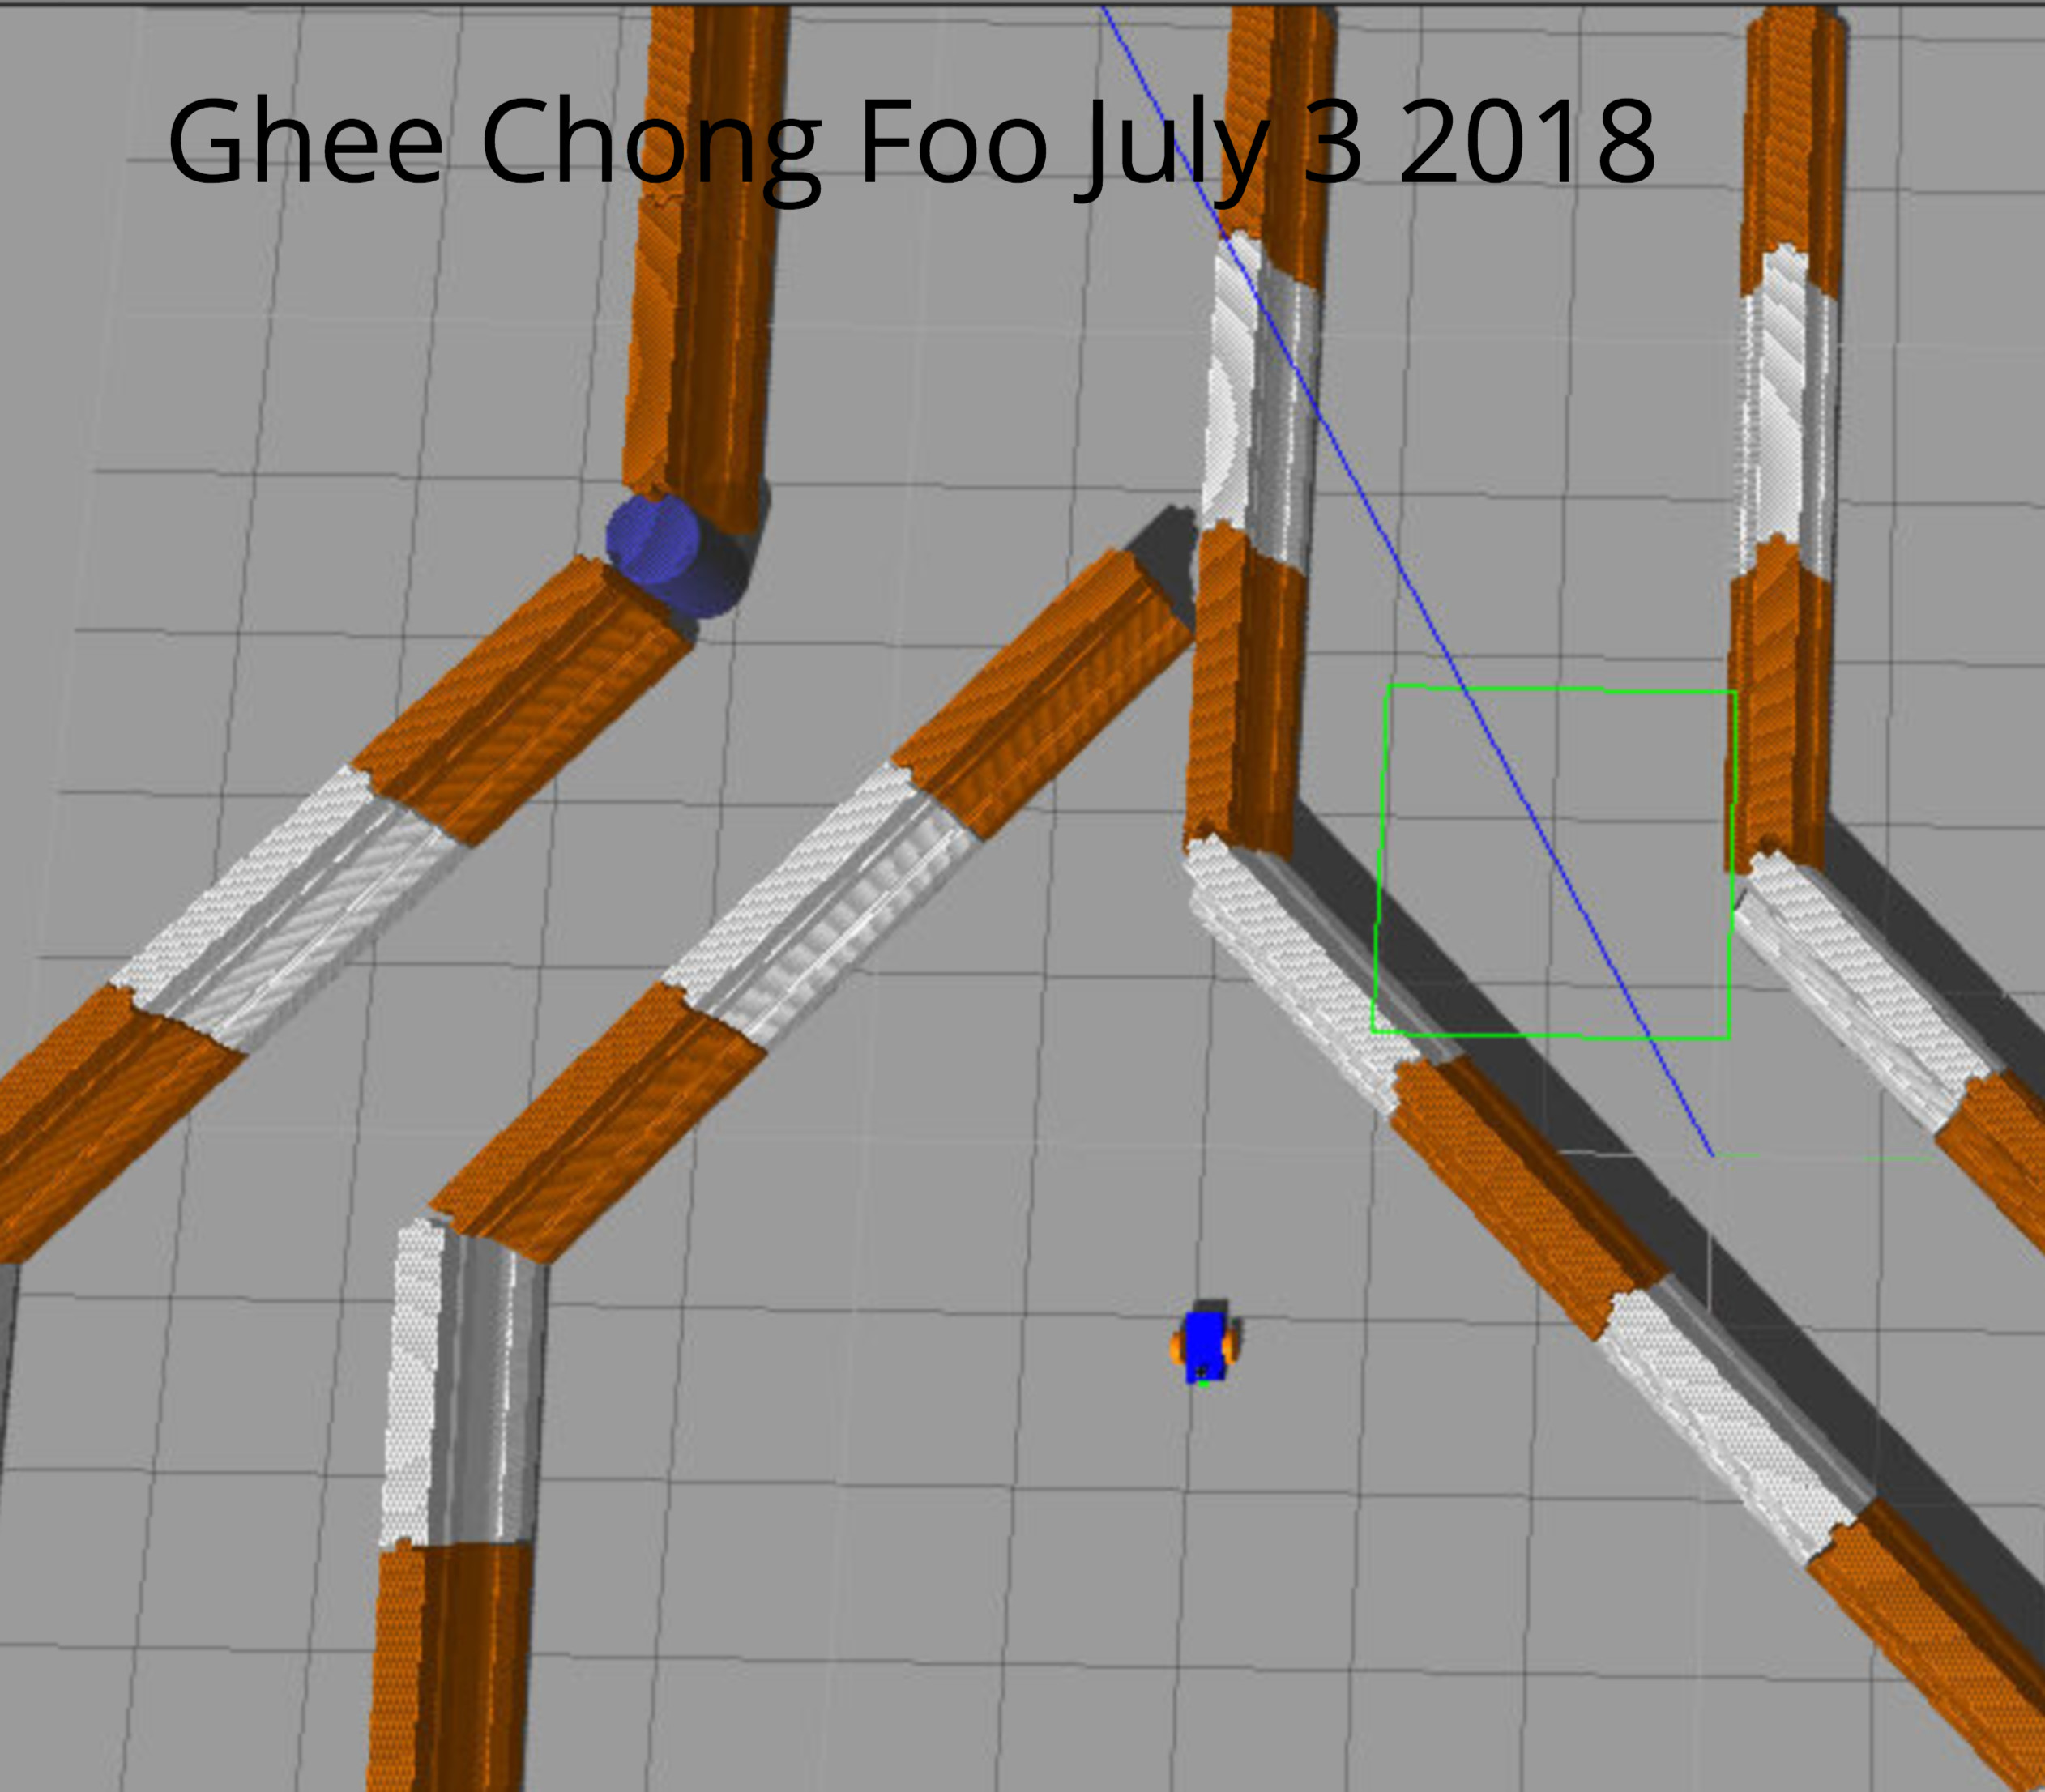
\includegraphics[width=\linewidth]{udacity_bot_reach_goal_gazebo}
      \caption{udacity\_bot reached goal Gazebo view}
      \label{fig:udacity_bot_reach_goal_gazebo}
\end{figure}

The benchmark model, namely udacity\_bot, was able to reach the goal within 2 minutes. The particles start to converge around 30 seconds.  In some run robot was uncertain of its position especially during turning of the corners, but still able to navigate to the final goal.

Video link showing udacity\_bot moving from initial position to goal:
\url{https://youtu.be/A2lqlh1FHoc}


\subsubsection{Student}

\begin{figure}[thpb]
      \centering
      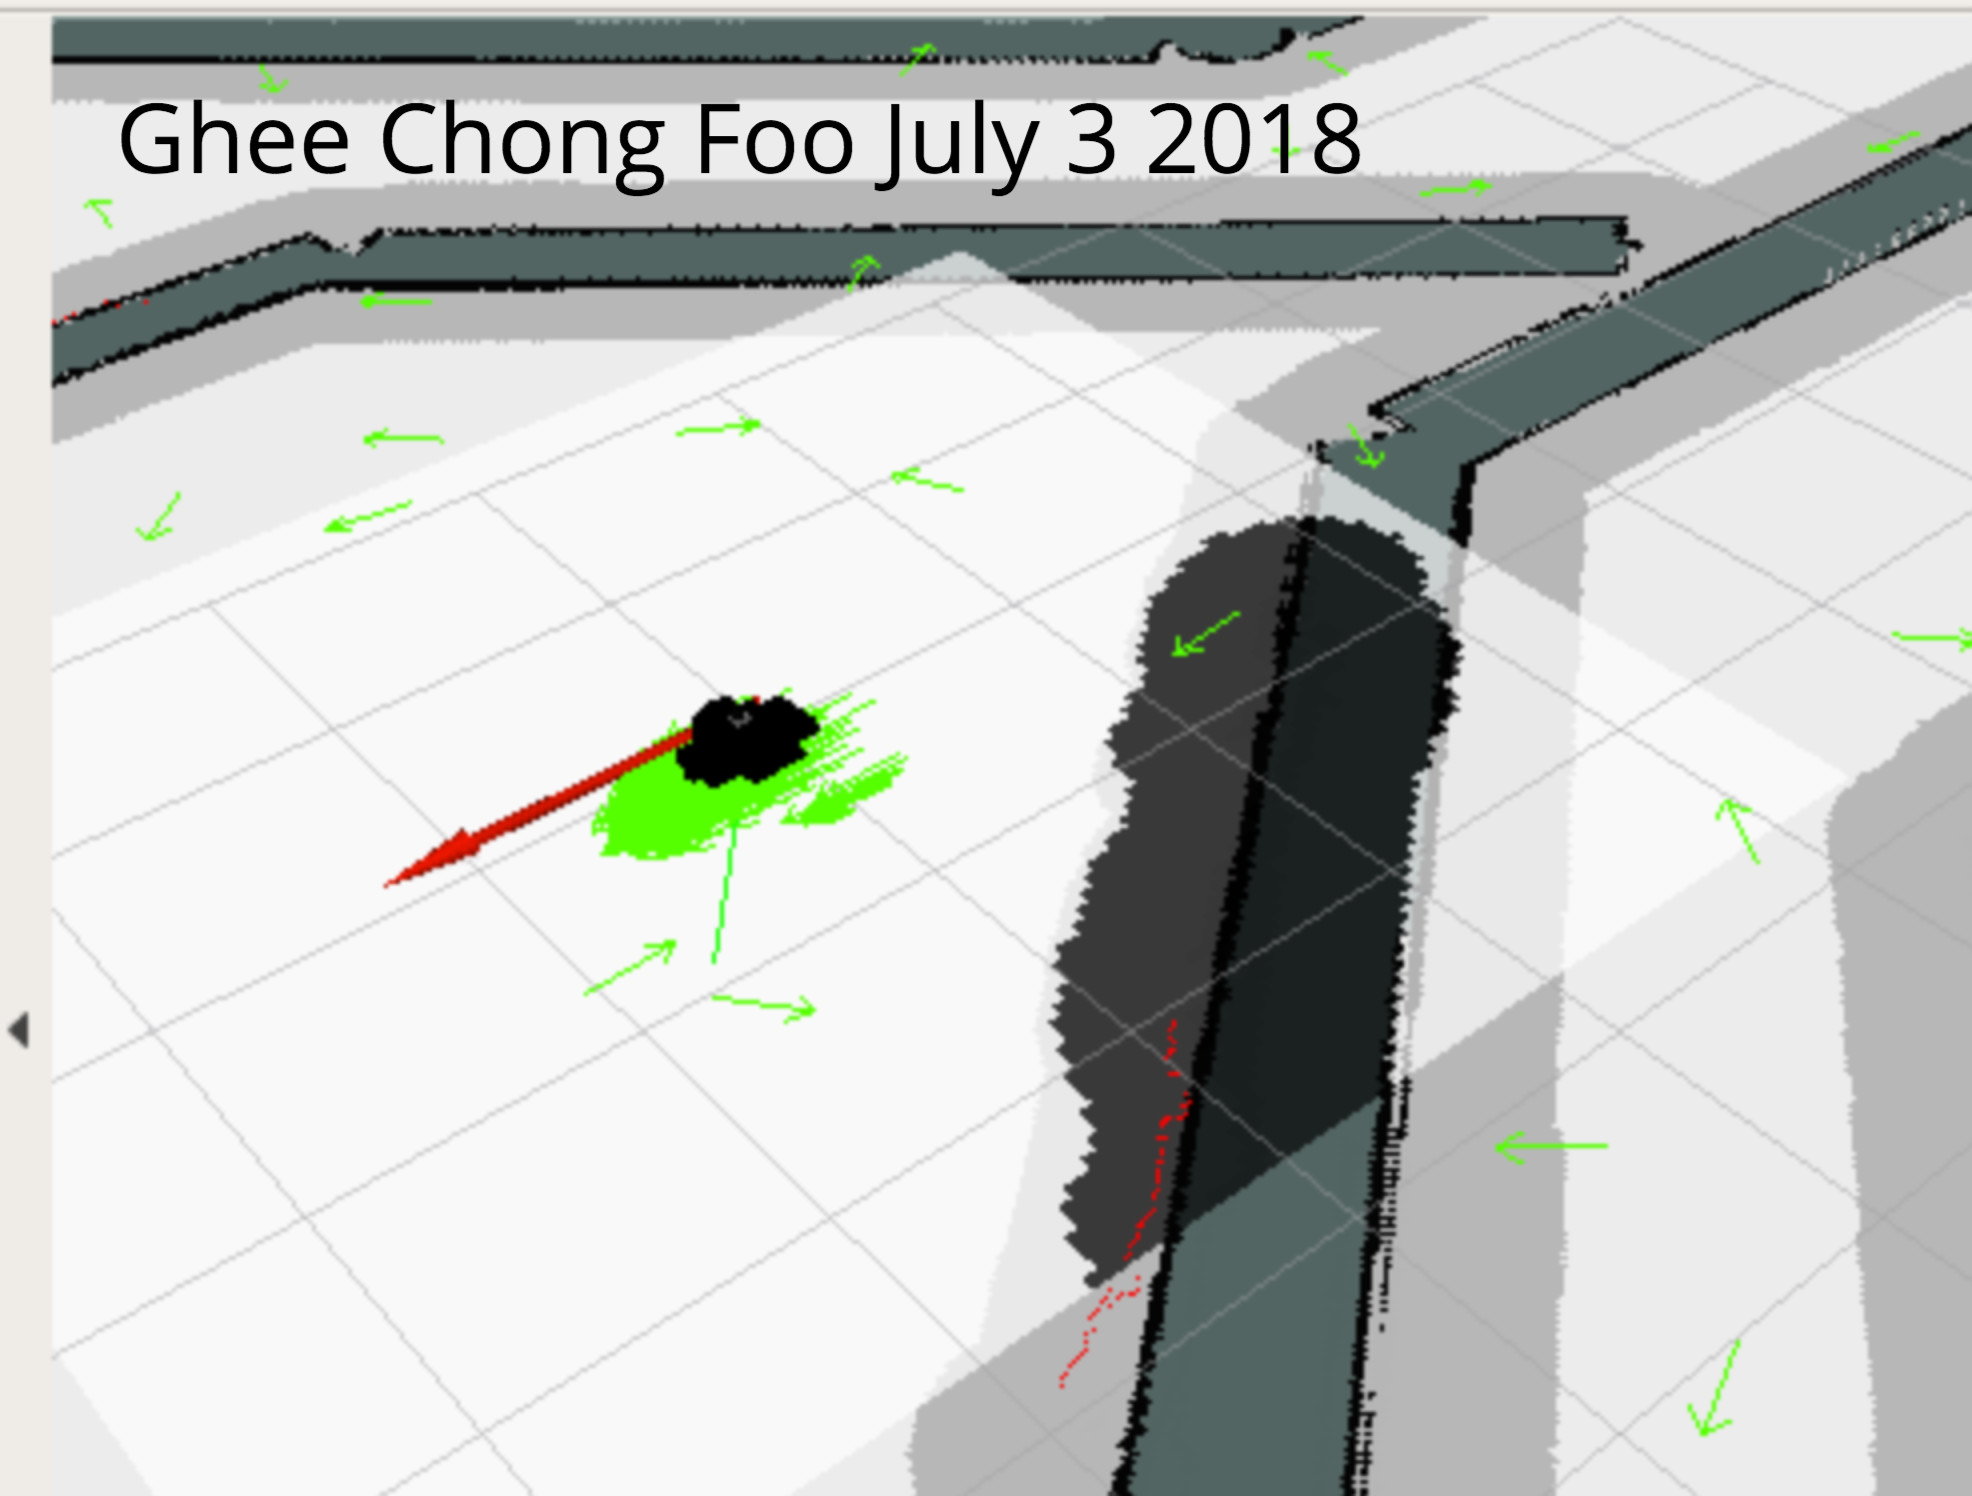
\includegraphics[width=\linewidth]{GC_bot_reach_goal_rviz}
      \caption{GC\_bot reached goal Rviz view}
      \label{fig:GC_bot_reach_goal_rviz}
\end{figure}

\begin{figure}[thpb]
      \centering
      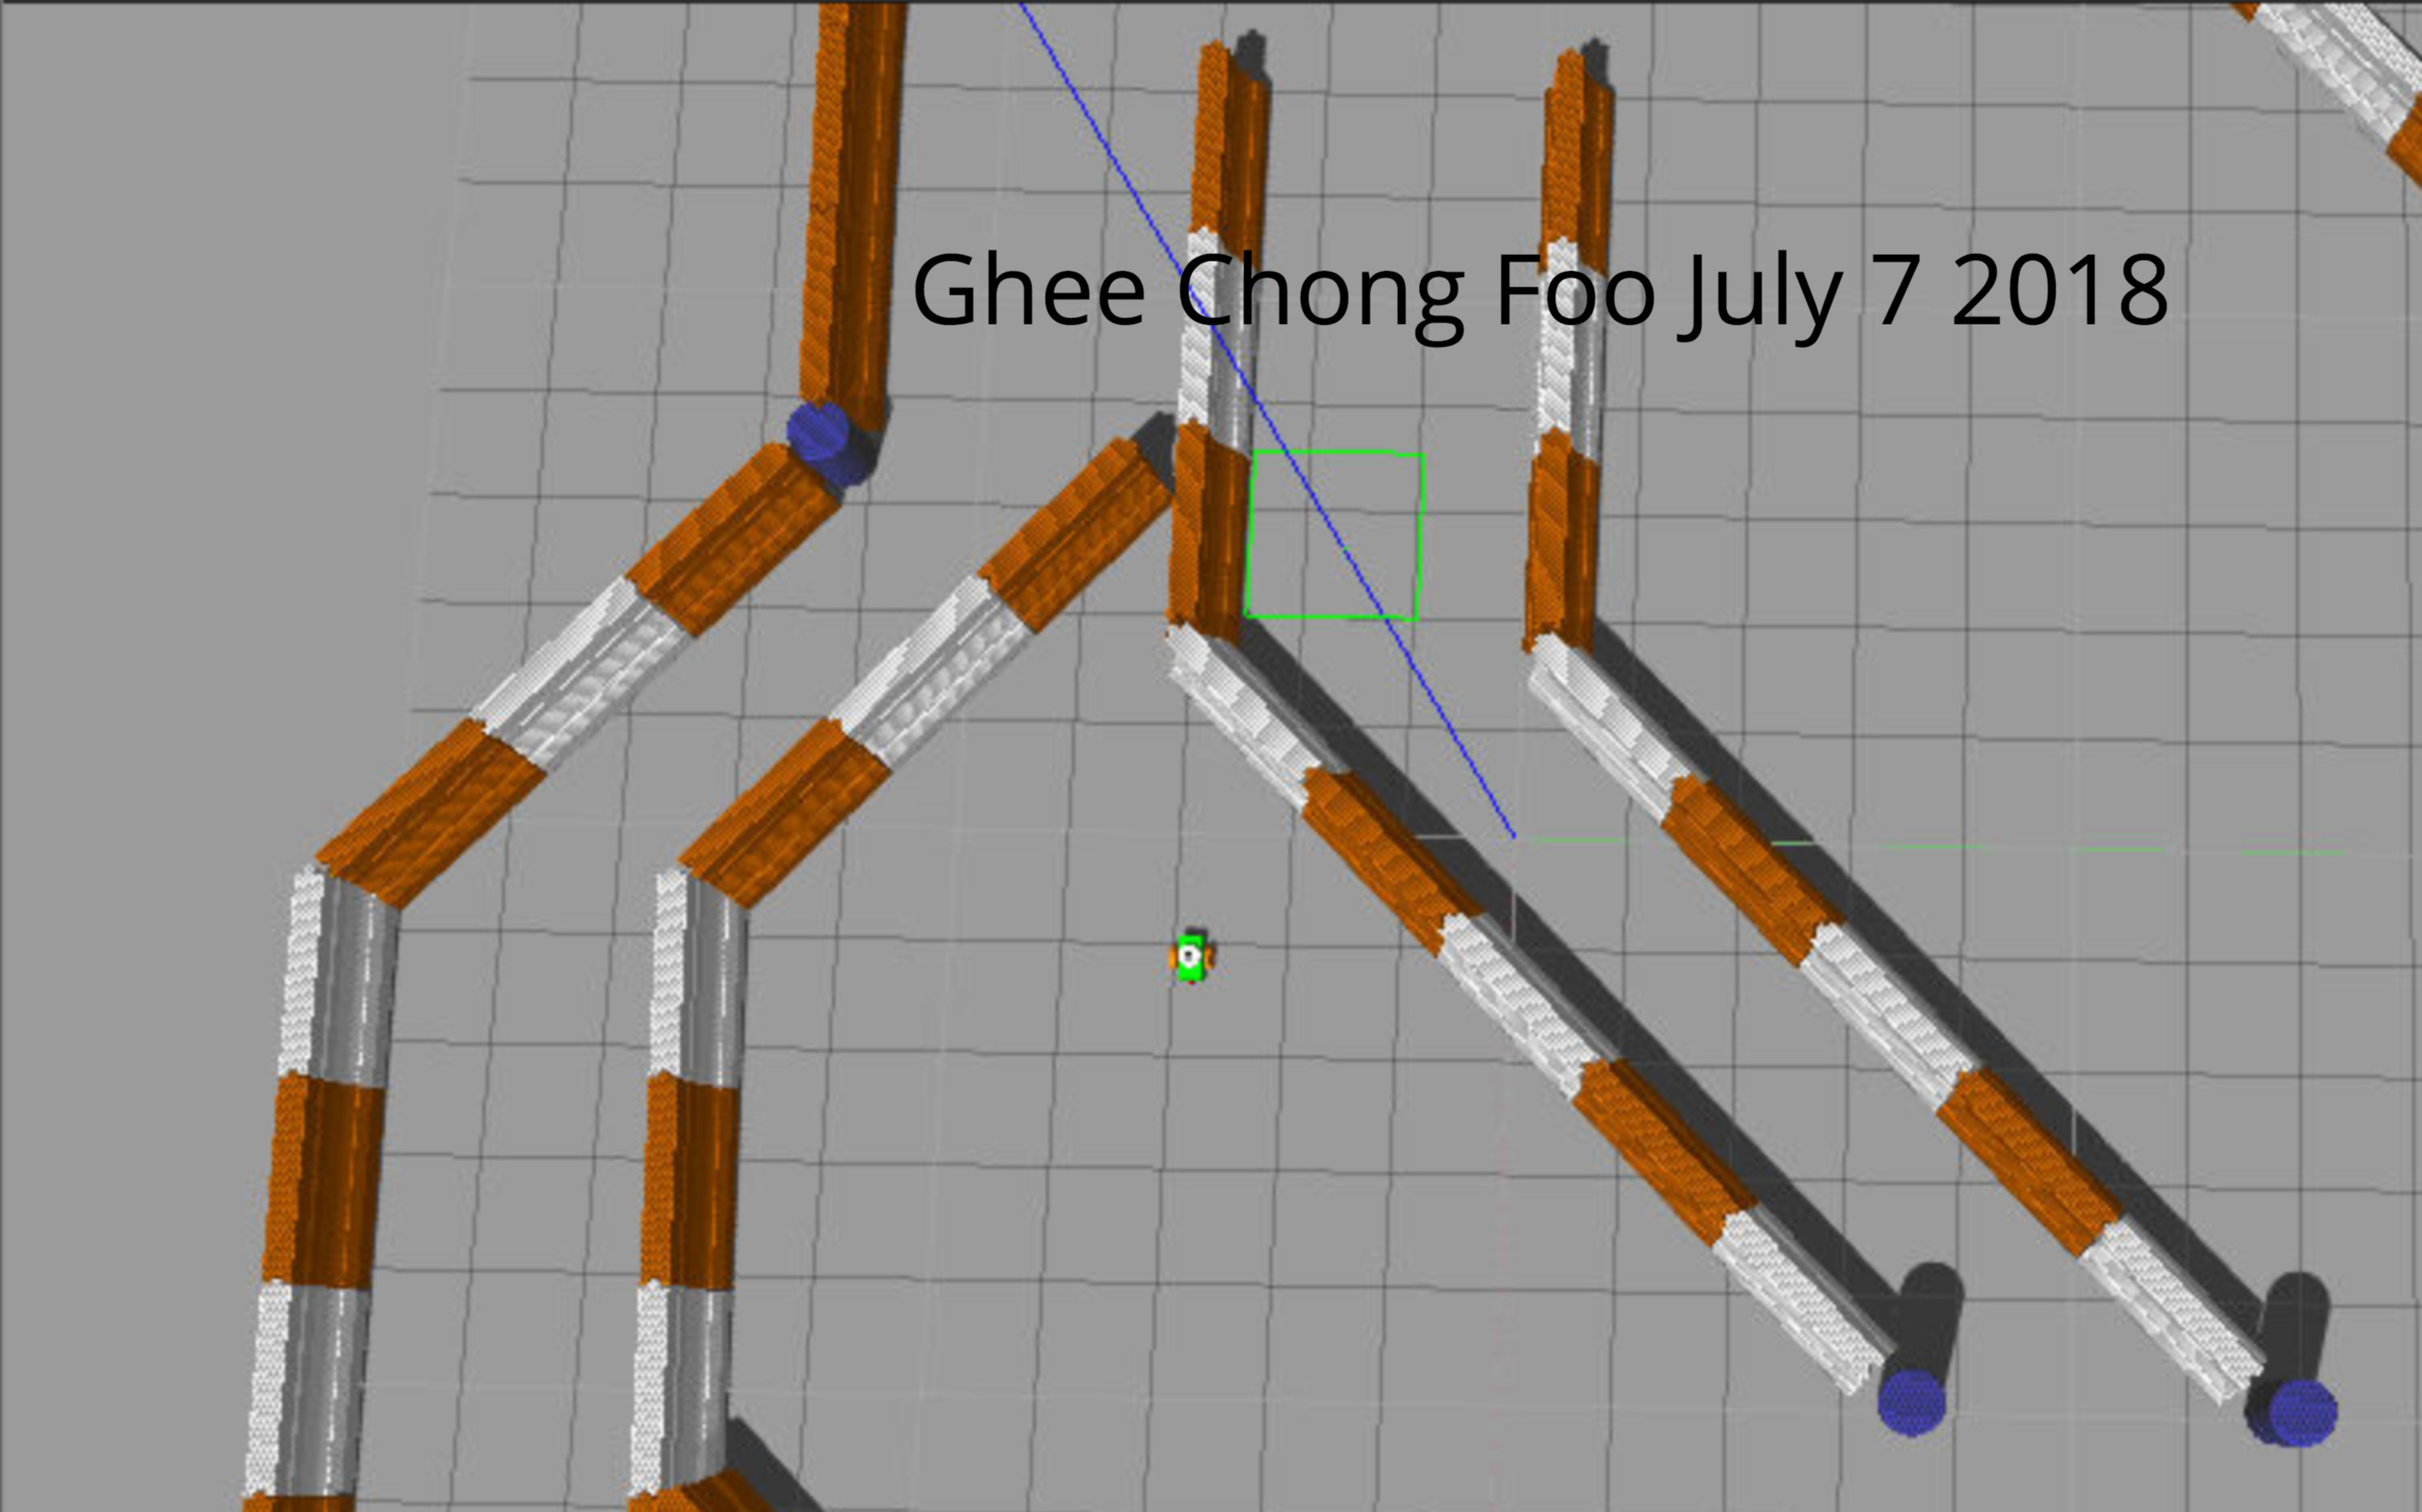
\includegraphics[width=\linewidth]{GC_bot_reach_goal_gazebo}
      \caption{GC\_bot reached goal Gazebo view}
      \label{fig:GC_bot_reach_goal_gazebo}
\end{figure}

The student model, i.e. GC\_bot, was able to reach the goal within 4 minutes, with particles start to converge after 90 seconds.  The robot is less certain of its position and making unnecessary turns during navigation. This can be concluded by observing the particles around the robot. The particles was more scattered even after it reached the goal, as depicted in Fig. \ref{fig:GC_bot_reach_goal_rviz}.

Video link showing GC\_bot moving from initial position to goal:
\url{https://youtu.be/3mdWm8pfrZw}

%\subsection{Technical Comparison} % only facts
%Discuss the difference of the layout, parameters, performance etc. between the benchmark robot and your robot. It is acceptable for your custom robot to perform worse than the provided robot. The focus is on learning and understanding, not performance. 

%GC\_bot perform worse than udacity\_bot in terms of navigation time and particle convergence.

\section{Discussion}
%This is the only section of the report where you may include your opinion. However, make sure your opinion is based on facts. If your robot performed poorly, make mention of what may be the underlying issues. If the robot runs well, which aspects contribute to that? Again, avoid writing in the first person (i.e. Do not use words like "I" or "me"). If you really find yourself struggling to avoid the word "I" or "me"; sometimes, this can be avoid with the use of the word “one”. As an example: instead of : "I think the robot cannot localize itself because the sensor does not provide enough information for localization" try: "one may believe the localization performance is poor because the sensor layout is not able to provide enough information for localization". They say the same thing, but the second avoids the first person. 

\subsection{Topics}
\begin{itemize}
%\item Which robot performed better?
\item The benchmark model perform better than student model
%\item Why it performed better? (opinion)
\item The benchmark model performed better because the sensor range was better tuned
%\item How would you approach the 'Kidnapped Robot' problem?
%\item What types of scenario could localization be performed?
%\item Where would you use MCL/AMCL in an industry domain?
\end {itemize}

\section{Conclusion / Future work}
%This section is intended to summarize your report. Your summary should include a recap of the results, did this project achieve what you attempted, how would you deploy it on hardware and how could this project be applied to commercial products? 
%For Future Work, address areas of work that you may not have addressed in your report as possible next steps. This could be due to time constraints, lack of currently developed methods / technology, and areas of application outside of your current implementation. Again, avoid the use of the first-person.

The robot model achieved the project goal of moving from initial position to the goal position and direction as specified.  There are wide range of usage for this kind of mobile robot application, e.g. transporting items from one area to another in factory/hospital/farm, which are often crowded with obstacles, and constant changes in environment.  The model can be further deployed in real hardware, e.g. mounting the Nvidia TX2 on a robot with real camera and sensors.  As this model was done in simulation mode, more fine tuning will be needed as real-world noise will inevitably creep in and make the robot moving more uncertain, if not fail to reach the goal.

%\subsection{Modifications for Improvement}
%Examples:
%\begin{itemize}
%\item Base Dimension
%\item Sensor Location
%\item Sensor Layout
%\item Sensor Amount
%\end{itemize}

%\subsection{Hardware Deployment}
%\begin{enumerate}
%\item What would need to be done?
%\item Computation time/resource considerations?
%\end{enumerate}



\bibliography{bib}
\bibliographystyle{ieeetr}

\end{document}